\section{UML Modeling and Design Patterns}
\label{sec:uml_modeling}

This section presents a comprehensive UML analysis of the Robotic Ultrasound System, highlighting the structural and behavioral aspects of the system through various diagram types and design pattern implementations.

\subsection{Class Diagrams}
\label{subsec:class_diagrams}

The system's object-oriented design is captured through detailed class diagrams that illustrate inheritance hierarchies, composition relationships, and interface implementations.

\subsubsection{Core USLib Class Structure}

\begin{figure}[h]
\centering
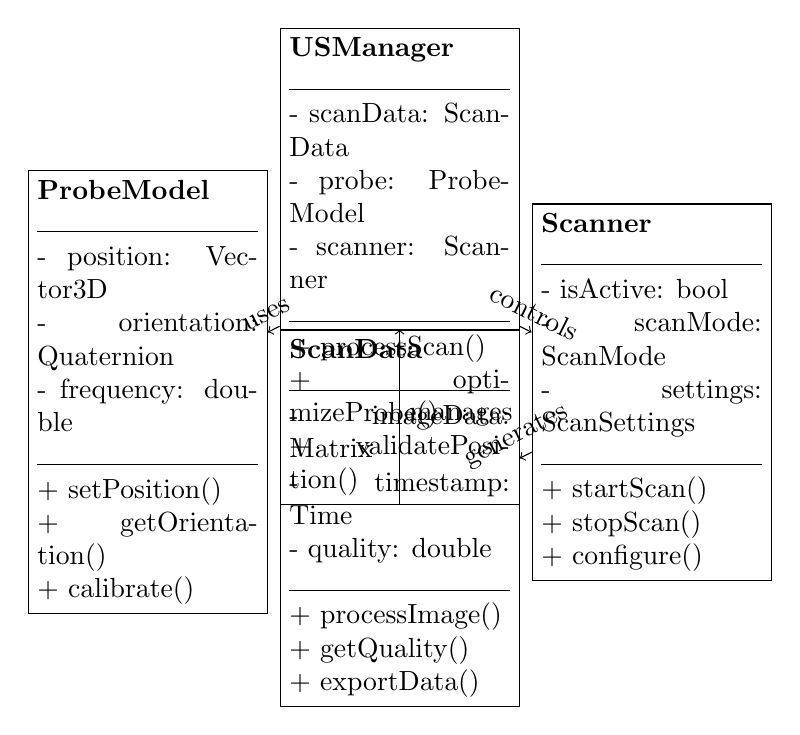
\begin{tikzpicture}[scale=0.8]
% USManager class
\node[draw, rectangle, minimum width=3cm, minimum height=2cm] (usmanager) at (0,4) {
    \begin{minipage}{2.8cm}
        \textbf{USManager}\\
        \rule{\linewidth}{0.4pt}\\
        - scanData: ScanData\\
        - probe: ProbeModel\\
        - scanner: Scanner\\
        \rule{\linewidth}{0.4pt}\\
        + processScan()\\
        + optimizeProbe()\\
        + validatePosition()
    \end{minipage}
};

% ProbeModel class
\node[draw, rectangle, minimum width=3cm, minimum height=1.8cm] (probe) at (-4,2) {
    \begin{minipage}{2.8cm}
        \textbf{ProbeModel}\\
        \rule{\linewidth}{0.4pt}\\
        - position: Vector3D\\
        - orientation: Quaternion\\
        - frequency: double\\
        \rule{\linewidth}{0.4pt}\\
        + setPosition()\\
        + getOrientation()\\
        + calibrate()
    \end{minipage}
};

% Scanner class
\node[draw, rectangle, minimum width=3cm, minimum height=1.8cm] (scanner) at (4,2) {
    \begin{minipage}{2.8cm}
        \textbf{Scanner}\\
        \rule{\linewidth}{0.4pt}\\
        - isActive: bool\\
        - scanMode: ScanMode\\
        - settings: ScanSettings\\
        \rule{\linewidth}{0.4pt}\\
        + startScan()\\
        + stopScan()\\
        + configure()
    \end{minipage}
};

% ScanData class
\node[draw, rectangle, minimum width=3cm, minimum height=1.8cm] (scandata) at (0,0) {
    \begin{minipage}{2.8cm}
        \textbf{ScanData}\\
        \rule{\linewidth}{0.4pt}\\
        - imageData: Matrix\\
        - timestamp: Time\\
        - quality: double\\
        \rule{\linewidth}{0.4pt}\\
        + processImage()\\
        + getQuality()\\
        + exportData()
    \end{minipage}
};

% Relationships
\draw[->] (usmanager) -- (probe) node[midway, above, sloped] {uses};
\draw[->] (usmanager) -- (scanner) node[midway, above, sloped] {controls};
\draw[->] (usmanager) -- (scandata) node[midway, right] {manages};
\draw[->] (scanner) -- (scandata) node[midway, above, sloped] {generates};

\end{tikzpicture}
\caption{Core USLib Class Relationships}
\label{fig:uslib_classes}
\end{figure}

\subsubsection{Trajectory Planning Hierarchy}

The trajectory planning subsystem demonstrates a clear inheritance hierarchy with abstract base classes and concrete implementations:

\begin{figure}[h]
\centering
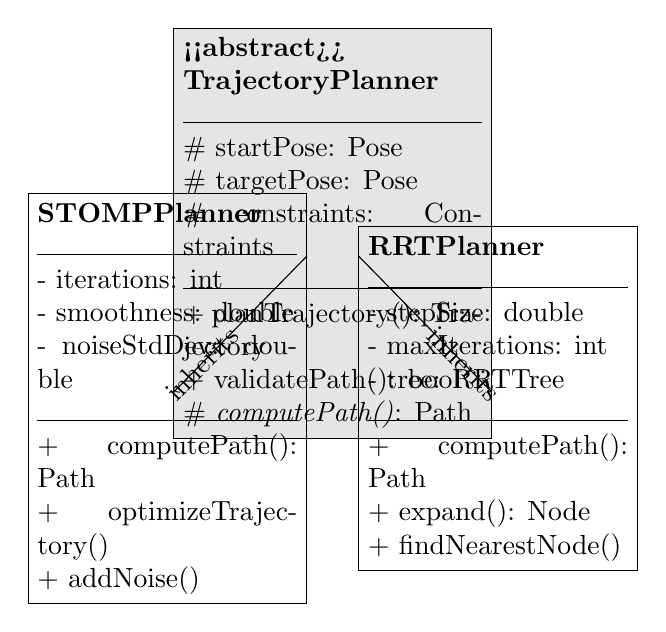
\begin{tikzpicture}[scale=0.7]
% Abstract base class
\node[draw, rectangle, minimum width=4cm, minimum height=2cm, fill=gray!20] (planner) at (0,4) {
    \begin{minipage}{3.8cm}
        \textbf{<<abstract>>}\\
        \textbf{TrajectoryPlanner}\\
        \rule{\linewidth}{0.4pt}\\
        \# startPose: Pose\\
        \# targetPose: Pose\\
        \# constraints: Constraints\\
        \rule{\linewidth}{0.4pt}\\
        + planTrajectory(): Trajectory\\
        + validatePath(): bool\\
        \# \textit{computePath()}: Path
    \end{minipage}
};

% STOMP implementation
\node[draw, rectangle, minimum width=3.5cm, minimum height=2cm] (stomp) at (-3,1) {
    \begin{minipage}{3.3cm}
        \textbf{STOMPPlanner}\\
        \rule{\linewidth}{0.4pt}\\
        - iterations: int\\
        - smoothness: double\\
        - noiseStdDev: double\\
        \rule{\linewidth}{0.4pt}\\
        + computePath(): Path\\
        + optimizeTrajectory()\\
        + addNoise()
    \end{minipage}
};

% RRT implementation
\node[draw, rectangle, minimum width=3.5cm, minimum height=2cm] (rrt) at (3,1) {
    \begin{minipage}{3.3cm}
        \textbf{RRTPlanner}\\
        \rule{\linewidth}{0.4pt}\\
        - stepSize: double\\
        - maxIterations: int\\
        - tree: RRTTree\\
        \rule{\linewidth}{0.4pt}\\
        + computePath(): Path\\
        + expand(): Node\\
        + findNearestNode()
    \end{minipage}
};

% Inheritance relationships
\draw[->] (stomp) -- (planner) node[midway, left, sloped] {inherits};
\draw[->] (rrt) -- (planner) node[midway, right, sloped] {inherits};

\end{tikzpicture}
\caption{Trajectory Planning Class Hierarchy}
\label{fig:trajectory_hierarchy}
\end{figure}

\subsection{Sequence Diagrams}
\label{subsec:sequence_diagrams}

Sequence diagrams illustrate the dynamic interactions between system components during key operational scenarios.

\subsubsection{Scan Optimization Sequence}

\begin{figure}[h]
\centering
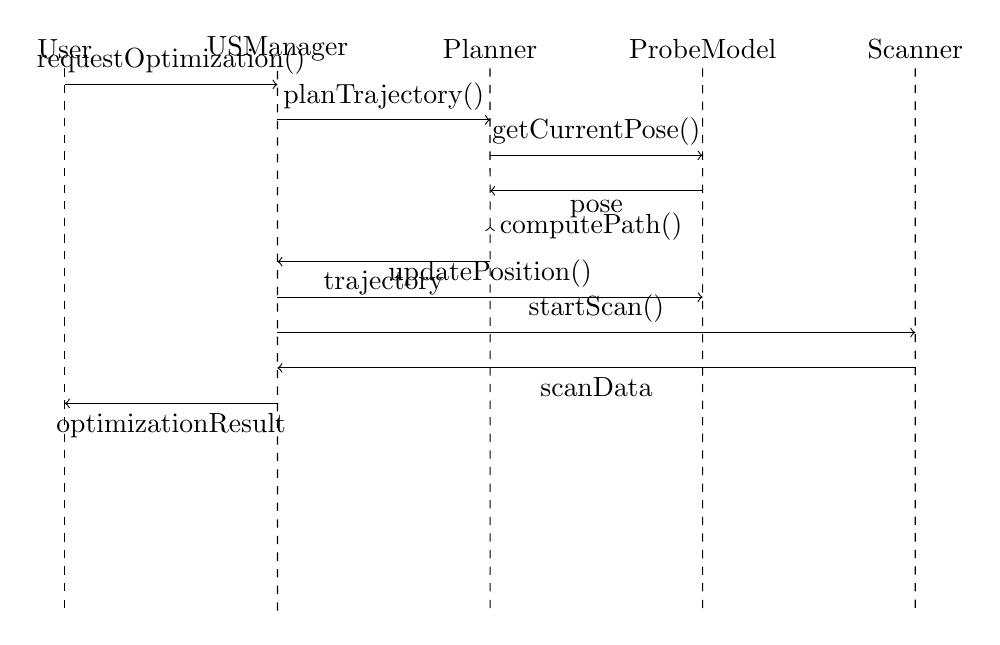
\begin{tikzpicture}[scale=0.9]
% Actors
\node (user) at (0,8) {User};
\node (manager) at (3,8) {USManager};
\node (planner) at (6,8) {Planner};
\node (probe) at (9,8) {ProbeModel};
\node (scanner) at (12,8) {Scanner};

% Lifelines
\draw[dashed] (user) -- (0,0);
\draw[dashed] (manager) -- (3,0);
\draw[dashed] (planner) -- (6,0);
\draw[dashed] (probe) -- (9,0);
\draw[dashed] (scanner) -- (12,0);

% Messages
\draw[->] (0,7.5) -- (3,7.5) node[midway, above] {requestOptimization()};
\draw[->] (3,7) -- (6,7) node[midway, above] {planTrajectory()};
\draw[->] (6,6.5) -- (9,6.5) node[midway, above] {getCurrentPose()};
\draw[<-] (6,6) -- (9,6) node[midway, below] {pose};
\draw[->] (6,5.5) -- (6,5.5) node[right] {computePath()};
\draw[<-] (3,5) -- (6,5) node[midway, below] {trajectory};
\draw[->] (3,4.5) -- (9,4.5) node[midway, above] {updatePosition()};
\draw[->] (3,4) -- (12,4) node[midway, above] {startScan()};
\draw[<-] (3,3.5) -- (12,3.5) node[midway, below] {scanData};
\draw[<-] (0,3) -- (3,3) node[midway, below] {optimizationResult};

\end{tikzpicture}
\caption{Scan Optimization Sequence}
\label{fig:scan_optimization_sequence}
\end{figure}

\subsection{State Diagrams}
\label{subsec:state_diagrams}

State diagrams model the behavioral states of key system components and their transitions.

\subsubsection{Scanner State Machine}

\begin{figure}[h]
\centering
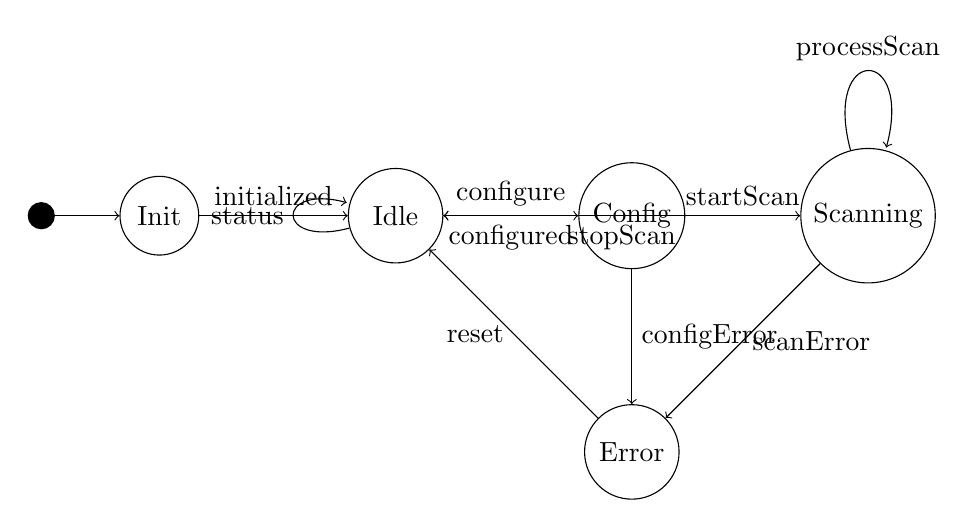
\begin{tikzpicture}[scale=1.0]
% States
\node[draw, circle, minimum size=1cm] (init) at (0,4) {Init};
\node[draw, circle, minimum size=1.2cm] (idle) at (3,4) {Idle};
\node[draw, circle, minimum size=1.2cm] (config) at (6,4) {Config};
\node[draw, circle, minimum size=1.2cm] (scanning) at (9,4) {Scanning};
\node[draw, circle, minimum size=1.2cm] (error) at (6,1) {Error};

% Initial state
\node[draw, circle, fill=black, minimum size=0.3cm] (start) at (-1.5,4) {};

% Transitions
\draw[->] (start) -- (init);
\draw[->] (init) -- (idle) node[midway, above] {initialized};
\draw[->] (idle) -- (config) node[midway, above] {configure};
\draw[->] (config) -- (idle) node[midway, below] {configured};
\draw[->] (config) -- (scanning) node[midway, above] {startScan};
\draw[->] (scanning) -- (idle) node[midway, below] {stopScan};
\draw[->] (config) -- (error) node[midway, right] {configError};
\draw[->] (scanning) -- (error) node[midway, right] {scanError};
\draw[->] (error) -- (idle) node[midway, left] {reset};

% Self-loops
\path (scanning) edge [loop above] node {processScan} (scanning);
\path (idle) edge [loop left] node {status} (idle);

\end{tikzpicture}
\caption{Scanner State Machine}
\label{fig:scanner_state_machine}
\end{figure}

\subsection{Activity Diagrams}
\label{subsec:activity_diagrams}

Activity diagrams capture the workflow and decision points in complex system processes.

\subsubsection{Trajectory Planning Workflow}

\begin{figure}[h]
\centering
\begin{tikzpicture}[scale=0.8]
% Start
\node[draw, circle, fill=black, minimum size=0.3cm] (start) at (0,10) {};

% Activities
\node[draw, rectangle, rounded corners, minimum width=3cm] (init) at (0,8.5) {Initialize Planner};
\node[draw, rectangle, rounded corners, minimum width=3cm] (validate) at (0,7) {Validate Input Poses};
\node[draw, diamond, minimum size=1cm] (valid) at (0,5.5) {Valid?};
\node[draw, rectangle, rounded corners, minimum width=3cm] (compute) at (0,4) {Compute Trajectory};
\node[draw, diamond, minimum size=1cm] (collision) at (0,2.5) {Collision Free?};
\node[draw, rectangle, rounded corners, minimum width=3cm] (optimize) at (3,2.5) {Optimize Path};
\node[draw, rectangle, rounded corners, minimum width=3cm] (error) at (-3,5.5) {Report Error};
\node[draw, rectangle, rounded corners, minimum width=3cm] (return) at (0,1) {Return Trajectory};

% End
\node[draw, circle, minimum size=0.3cm] (end) at (0,-0.5) {};
\node[draw, circle, fill=black, minimum size=0.2cm] at (0,-0.5) {};

% Flows
\draw[->] (start) -- (init);
\draw[->] (init) -- (validate);
\draw[->] (validate) -- (valid);
\draw[->] (valid) -- (compute) node[midway, right] {Yes};
\draw[->] (valid) -- (error) node[midway, above] {No};
\draw[->] (compute) -- (collision);
\draw[->] (collision) -- (optimize) node[midway, above] {No};
\draw[->] (collision) -- (return) node[midway, right] {Yes};
\draw[->] (optimize) -- (compute);
\draw[->] (return) -- (end);
\draw[->] (error) -- (end);

\end{tikzpicture}
\caption{Trajectory Planning Activity Workflow}
\label{fig:trajectory_planning_activity}
\end{figure}

\subsection{Design Patterns Implementation}
\label{subsec:design_patterns}

The system extensively uses well-established design patterns to ensure maintainability, extensibility, and testability.

\subsubsection{Strategy Pattern in Trajectory Planning}

The trajectory planning subsystem implements the Strategy pattern to allow runtime selection of different planning algorithms:

\begin{lstlisting}[language=C++, caption=Strategy Pattern Implementation]
// Abstract strategy interface
class TrajectoryPlannerStrategy {
public:
    virtual ~TrajectoryPlannerStrategy() = default;
    virtual Trajectory plan(const Pose& start, 
                          const Pose& goal, 
                          const Constraints& constraints) = 0;
};

// Concrete strategies
class STOMPStrategy : public TrajectoryPlannerStrategy {
public:
    Trajectory plan(const Pose& start, const Pose& goal, 
                   const Constraints& constraints) override {
        // STOMP-specific implementation
        return stompPlanner.computeTrajectory(start, goal, constraints);
    }
};

class RRTStrategy : public TrajectoryPlannerStrategy {
public:
    Trajectory plan(const Pose& start, const Pose& goal, 
                   const Constraints& constraints) override {
        // RRT-specific implementation
        return rrtPlanner.expandTree(start, goal, constraints);
    }
};

// Context class
class TrajectoryPlannerContext {
private:
    std::unique_ptr<TrajectoryPlannerStrategy> strategy_;
public:
    void setStrategy(std::unique_ptr<TrajectoryPlannerStrategy> strategy) {
        strategy_ = std::move(strategy);
    }
    
    Trajectory planTrajectory(const Pose& start, const Pose& goal, 
                            const Constraints& constraints) {
        return strategy_->plan(start, goal, constraints);
    }
};
\end{lstlisting}

\subsubsection{Observer Pattern for Event Handling}

The system uses the Observer pattern for decoupled event notification across components:

\begin{lstlisting}[language=C++, caption=Observer Pattern for Events]
// Abstract observer interface
class ScanEventObserver {
public:
    virtual ~ScanEventObserver() = default;
    virtual void onScanStarted(const ScanEvent& event) {}
    virtual void onScanCompleted(const ScanEvent& event) {}
    virtual void onScanError(const ScanEvent& event) {}
};

// Subject class
class Scanner {
private:
    std::vector<std::weak_ptr<ScanEventObserver>> observers_;
    
public:
    void addObserver(std::shared_ptr<ScanEventObserver> observer) {
        observers_.push_back(observer);
    }
    
    void notifyObservers(const ScanEvent& event, EventType type) {
        auto it = observers_.begin();
        while (it != observers_.end()) {
            if (auto observer = it->lock()) {
                switch (type) {
                    case EventType::SCAN_STARTED:
                        observer->onScanStarted(event);
                        break;
                    case EventType::SCAN_COMPLETED:
                        observer->onScanCompleted(event);
                        break;
                    case EventType::SCAN_ERROR:
                        observer->onScanError(event);
                        break;
                }
                ++it;
            } else {
                it = observers_.erase(it);
            }
        }
    }
};
\end{lstlisting}

\subsubsection{Factory Pattern for Component Creation}

A factory pattern manages the creation of different component types:

\begin{lstlisting}[language=C++, caption=Factory Pattern Implementation]
// Abstract factory
class USComponentFactory {
public:
    virtual ~USComponentFactory() = default;
    virtual std::unique_ptr<ProbeModel> createProbe(ProbeType type) = 0;
    virtual std::unique_ptr<Scanner> createScanner(ScannerType type) = 0;
    virtual std::unique_ptr<TrajectoryPlanner> createPlanner(PlannerType type) = 0;
};

// Concrete factory
class DefaultUSComponentFactory : public USComponentFactory {
public:
    std::unique_ptr<ProbeModel> createProbe(ProbeType type) override {
        switch (type) {
            case ProbeType::LINEAR:
                return std::make_unique<LinearProbe>();
            case ProbeType::CURVED:
                return std::make_unique<CurvedProbe>();
            case ProbeType::PHASED_ARRAY:
                return std::make_unique<PhasedArrayProbe>();
            default:
                throw std::invalid_argument("Unknown probe type");
        }
    }
    
    std::unique_ptr<Scanner> createScanner(ScannerType type) override {
        switch (type) {
            case ScannerType::HIGH_FREQUENCY:
                return std::make_unique<HighFrequencyScanner>();
            case ScannerType::DOPPLER:
                return std::make_unique<DopplerScanner>();
            default:
                throw std::invalid_argument("Unknown scanner type");
        }
    }
    
    std::unique_ptr<TrajectoryPlanner> createPlanner(PlannerType type) override {
        switch (type) {
            case PlannerType::STOMP:
                return std::make_unique<STOMPPlanner>();
            case PlannerType::RRT:
                return std::make_unique<RRTPlanner>();
            default:
                throw std::invalid_argument("Unknown planner type");
        }
    }
};
\end{lstlisting}

\subsection{Component Interaction Patterns}
\label{subsec:interaction_patterns}

The system demonstrates several sophisticated interaction patterns that promote loose coupling and high cohesion.

\subsubsection{Publish-Subscribe Pattern}

For asynchronous communication between system components:

\begin{lstlisting}[language=C++, caption=Publish-Subscribe Implementation]
template<typename EventType>
class EventBus {
private:
    std::unordered_map<std::string, 
        std::vector<std::function<void(const EventType&)>>> subscribers_;
    std::mutex mutex_;
    
public:
    void subscribe(const std::string& topic, 
                  std::function<void(const EventType&)> callback) {
        std::lock_guard<std::mutex> lock(mutex_);
        subscribers_[topic].push_back(callback);
    }
    
    void publish(const std::string& topic, const EventType& event) {
        std::lock_guard<std::mutex> lock(mutex_);
        if (auto it = subscribers_.find(topic); it != subscribers_.end()) {
            for (const auto& callback : it->second) {
                callback(event);
            }
        }
    }
};

// Usage example
EventBus<ScanData> scanDataBus;

// Subscribe to scan events
scanDataBus.subscribe("scan_completed", 
    [](const ScanData& data) {
        processCompletedScan(data);
    });

// Publish scan completion
scanDataBus.publish("scan_completed", scanResult);
\end{lstlisting}

This comprehensive UML modeling demonstrates the system's sophisticated object-oriented design, clear separation of concerns, and adherence to established design patterns that ensure maintainability and extensibility.
